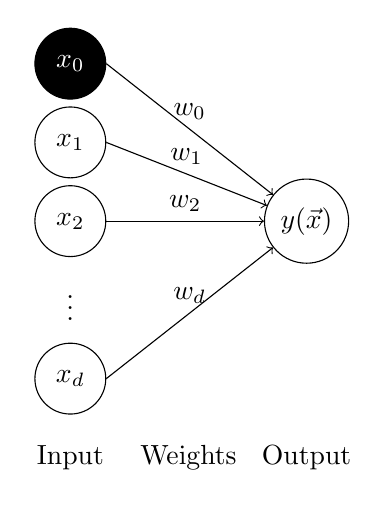
\begin{tikzpicture}[
	perceptron size/.style={minimum size=0.9cm},
	bias perceptron/.style={fill=black,text=white},
	perceptron/.style]
	
	% input perceptrons
	\node[draw, circle, perceptron size, bias perceptron] (0) at (0,4 cm) {$x_0$};
	\foreach \y/\ytext in {0/d, 2/2, 3/1}
		\node[draw, circle, perceptron size, perceptron] (\ytext) at (0,\y cm) {$x_\ytext$};
	\node at (0,1cm) {$\vdots$};

	% output perceptron
	\node[draw, circle, perceptron size] (y) at (3cm,2cm) {$y(\vec{x})$};

	% weights and connections
	\foreach \perceptron in {0, 1, 2, d}
		\draw[->] (\perceptron.east) -- node[above] {$w_\perceptron$} (y);

	% labeling
	\node at (0,-1cm) {Input};
	\node at (1.5cm,-1cm) {Weights};
	\node at (3cm,-1cm) {Output};
\end{tikzpicture}
